% interactcadsample.tex
% v1.03 - April 2017

\documentclass[]{interact}

\usepackage{epstopdf}% To incorporate .eps illustrations using PDFLaTeX, etc.
\usepackage{subfigure}% Support for small, `sub' figures and tables
\usepackage[russian]{babel}
%\usepackage[nolists,tablesfirst]{endfloat}% To `separate' figures and tables from text if required

\usepackage{natbib}% Citation support using natbib.sty
\bibpunct[, ]{(}{)}{;}{a}{}{,}% Citation support using natbib.sty
\renewcommand\bibfont{\fontsize{10}{12}\selectfont}% Bibliography support using natbib.sty

\theoremstyle{plain}% Theorem-like structures provided by amsthm.sty
\newtheorem{theorem}{Theorem}[section]
\newtheorem{lemma}[theorem]{Lemma}
\newtheorem{corollary}[theorem]{Corollary}
\newtheorem{proposition}[theorem]{Proposition}

\theoremstyle{definition}
\newtheorem{definition}[theorem]{Definition}
\newtheorem{example}[theorem]{Example}

\theoremstyle{remark}
\newtheorem{remark}{Remark}
\newtheorem{notation}{Notation}

\begin{document}

\articletype{Перевод и компиляция}

\title{Энтропия и выявление аномалий сетевого трафика}

\author{
\name{Волков Д.В.}
}

\maketitle

\begin{abstract}
В этой статье освещаются методы детекции сетевых аномалий, основанные на использовании энтропии -- основной характеристики систем с точки зрения теории информации. Также обсуждаются некоторые способы обнаружения аномалий временных рядов.
\end{abstract}

\begin{keywords}
Теория информации; энтропия; временные ряды; детекция аномалий; сетевая безопасность
\end{keywords}


\section{Introduction}

Использован материал нескольких статей:
\begin{itemize}
    \item On Detecting Abrupt Changes in Network Entropy Time Series,
    \item On selection of attributes for entropy based detection of DDoS,
    \item Information Metrics for Low-rate DDoS Attack Detection.
\end{itemize}

За последнее десятилетие большое количество исследований было сосредоточено на энтропии как мере «хаоса», присущего различным характеристикам сетевого трафика. В частности, энтропийные временные ряды оказались относительно хорошим методом обнаружения аномалий в сетевом трафике. К плюсам такого подхода относятся:
\begin{itemize}
    \item Масштабируемость. Предложенные методы способны использовать агрегированые данные (например, записи Netflow), что делает возможным использование в сколь угодно сложных и высоконагруженных сетях.
    \item Чувствительность к изменениям распределений характеристик трафика. Энтропийный подход помогает среагировать на аномалию и в тех случаях, когда такие классические характеристики трафика, как packets rate (rps) не обнаруживают значимого аномального поведения (т.о., способен выявлять атаки с низким относительным packets rate).
    \item Относительная легкость реализации и доступная интерпретация.
\end{itemize}

\subsection{Сетевые потоки}\label{class}

Итак, предлагаемые системы обнаружения аномалий на основе понятия <<энтропия>> анализируют сетевые потоки, а не отдельные сетевые пакеты.
Определим сетевые потоки (далее просто потоки) как однонаправленную метаинформацию о сетевых пакетах, имеющих следующие одинаковые характеристики: исходный и целевой IP-адрес и порты, а также тип протокола IP. Важно отметить, что вся сетевая активность в OSI
уровня 3 и выше сводится к потокам, т.е. не только TCP-соединения, но и протоколы без сохранения состояния, такие как UDP и ICMP.
Преимущества использования концепции потоков:
\begin{itemize}
    \item Они очень легкие (с точки зрения используемой и хранимой информации), что облегчает анализ.
    \item Вызывают меньше проблем с конфиденциальностью и персональными данными.
    \item Легко наладить доступ к необходимой информации в сети, например в виде Cisco NetFlow, sflow, или даже IPFIX (по вкусу).
\end{itemize}


\subsection{Энтропия}
Понятия энтропии в статистической физике и теории информации довольно близки друг другу. Кроме того, для нас будет фактом не последней важности при использовании именно энтропии как меры распределения характеристик трафика то, что энтропия также служит мерой близости состояния системы к равновесному (в теории неравновесных процессов, к коим можно относить и обмен сетевым трафиком). Как многие помнят, классическая энтропия Шеннона определяется как
\begin{equation}
    H = - \sum^n_{i=1} p_i \log p_i,
\end{equation}
где $p_i$ - вероятность $i$-го состояния системы, $n$ - количество всех возможных состояний системы. Чтобы облегчить интерпретацию результата и исключить влияние сезонных факторов, изменяющих $n$, будем использовать в дальнейшем нормализованную энтропию Шеннона
\begin{equation}
    H_0 = \frac{H}{\log n}, \longrightarrow H_0 \in [0, 1].
\end{equation}

\subsection{Атрибуты сетевого трафика и энтропийные временные ряды}

Теперь осталось пояснить, как именно мы будем вычислять [2] для различных характеристик сетевого трафика, и главное -- для каких?
Различные авторы предлагают использовать самые различные характеристики, однако практически во всех работах остаётся следующий основной набор:
\begin{itemize}
    \item Source IP,
    \item Destination IP,
    \item Source port,
    \item Destination port.
\end{itemize}
 Его предлагается иногда расширять с помощью других характеристик, например, Flow records или IP protocol для магистральных потоков.

 Мы будем использовать временные ряды величины $H_0$, вычисляемой для этих характеристик трафика, внутри временных окон конечной длины. Характерные длины окон (можно использовать перекрывающеся скользящие) -- это около 5-10 минут, из соображений того, что характерная продолжительность атаки на сетевую инфраструктуру это десятки минут, а также необходимость в достаточно большом количестве накопленной статистики.
 Итак, если нас интересует энтропия для IP адреса источника, тогда $n$ равно количеству уникальных IP адресов в окне, а что касается расчета вероятностей, то подавляющее большинство авторов используют количество пакетов с данной характеристикой как меру вероятности такого пакета в сети (что, в общем, логично, однако можно [иногда предлагается] использовать и количество байт, и количество потоков). Например, если у нас было 100 пакетов для 1.1.1.1, 100 пакетов для 1.1.1.2, и 300 пакетов для 2.2.2.2, то
 \begin{equation}
     p_{1.1.1.1} = p_{1.1.1.2} = \frac{100}{100 + 100 + 300} = 0.2
 \end{equation}
 \begin{equation}
     p_{2.2.2.2} = \frac{300}{500} = 0.6
 \end{equation}
 \begin{equation}
     H = -(0.2 \log 0.2 + 0.2 \log 0.2 + 0.6 \log 0.6) \approx 1.37
 \end{equation}
 \begin{equation}
     H_0 = \frac{1.37}{log 3} \approx 0.86.
 \end{equation}

 Далее мы обсудим, какие атрибуты и когда имеет смысл рассматривать (при каких интересующих типах атак).


\subsection{Feature selection}
В большинстве исследований, связанных с энтропией и сетевыми аномалиями, исследователи сосредоточились на IP-адресе источника, и соответственно, его распределении и энтропии. В общем случае это довольно хороший выбор.

В исследовании [ссылка] авторы экспериментировали с разными типами атак и проанализировали полезность различных атрибутов для обнаружения этих атак с помощью энтропийного подхода. А именно, был использован датасет NUST. Типы атак: TCP-SYN флуд, UDP флуд и Smurf. Для анализа было взято порядка 100 тыс. пакетов нормального трафика, и 10 тыс. пакетов атакованного трафика. Атрибутами являлись Source IP, Destination IP, Source Port and Destination Port (стандартные), но также рассматривались Flags (распределение по TCP-флагам), Length (распределение по длинам пакетов), Protocol (по протоколам).

В результате выяснилось, что полезно использовать в системах обнаружения аномалий на основе энтропийного подхода также и вышеупомянутые дополнительные к стандартным атрибуты, такие как длина пакета (очень хорошие результаты в случае TCP-SYN атак). Использовать энтропию по протоколам представляется относительно полезным, т.к. значимые результаты это принесло только в специфических случаях наподобие UDP флуда, но подобные типы атак легко могут быть обнаружены совсем традиционными методами слежения за трафиком.



\section{Алгоритм обнаружения сетевых аномалий на основе энтропийных временных рядов}

Данный метод представляет обобщение предлагаемого авторами [ссылка]. Обобщения затрагивают в основном то, какие атрибуты использовать для построения системы временных рядов, а также методы выявления аномалий конкретных временных рядов.

\subsection{Алгоритм}

\begin{enumerate}
    \item Выбираем, какие атрибуты будут использованы для построения энтропийных временных рядов. В [link] это стандартная четверка Src-Dst IP/Port, плюс распределение по flow records (1 flow records = Src IP + Dst IP + Src Port + Dst Port + IP Protocol).
    \item Строим временные ряды для нормализованных энтропий Шеннона! Необходимо накопить некоторую статистику за период, покрывающий основные сезонные факторы сети. В большинстве случаев можно ограничиться сутками. Обозначим множество рядов как $T$.
    \item Теперь для каждого временного ряда известна дисперсия за опорный интервал (так мы будем называть интервал для расчета дисперсии временного ряда в недавнем прошлом). Начиная со следующих моментов времени, наша система готова к обнаружению аномалий. $\sigma_i$ - дисперсия $i$-го временного ряда из $T$.
    \item Основная идея обнаружения резких изменений состоит в том, чтобы постоянно проводить краткосрочные прогнозы и определять разницу между прогнозом и фактическим значением. Авторы [ссылка] предлагают метод простого экспоненциального сглаживания, однако вам ничего не мешает взять что-то более сложное (и точное), от ARIMA до LSTM-сетей. \\
    Для каждого $T_i$ определяем ошибку прогноза на интересующий нас момент $t$:
    \begin{equation}
        \delta_i = | \texttt{Pred}(T_i(t)) - T_i(t) |.
    \end{equation}
    \item Однако определенные ошибки предсказаний не равны по своей значимости, потому что базовые временные ряды имеют разные дисперсии. По этой причине мы нормализуем ошибки предсказания относительно дисперсии соответствующих временных рядов, умножая на весовой коэффициент
    \begin{equation}
        w_i = \frac{1}{\sigma_i} \cdot \max (\sigma_1, \ldots, \sigma_n).
    \end{equation}
    \item Чтобы упростить процесс детекции аномалий, введем совокупную характеристику <<anomaly score>>:
    \begin{equation}
        AS = \sum_{i=1}^n \delta_i \cdot w_i.
    \end{equation}
    \item Если $AS > AS_{thr}$, говорим, что зафиксирована некая аномалия сетевого трафика. Величина $AS_{thr}$ определяется эмпирически в зависимости от количества базовых временных рядов $n$, а также требований к чувствительности детектора.

\end{enumerate}

\subsection{О настройке параметров}
Для нашего алгоритма необходимо установить несколько параметров. Каждая комбинация параметров связана с компромиссом: высокий уровень обнаружения за счет множества ложных срабатываний или наоборот.

\begin{itemize}
    \item \textbf{Длина скользящего окна.} Здесь речь идет о размере интервала, на котором вычисляются точечные значения энтропийных временных рядов. Маленькие окна очень чувствительны, и с одной стороны, это увеличит скорость обнаружения. С другой стороны, частота ложных тревог также увеличится. Большие окна сравнительно нечувствительны, что приводит к обратному эффекту. В качестве компромисса используют окна от 5 до 10 минут.
    \item \textbf{Размер перекрытия скользящих окон.} Перекрытие скользящих окон приводит к более детализированным временным рядам. Мы хотим заставить нашу систему как можно быстрее реагировать на резкие изменения, и поэтому мы выбрали относительное перекрытие в $80\%$.
    \item \textbf{Размер скользящего окна для расчета дисперсий.} Мы решили установить размер скользящего окна для расчета стандартного отклонения до 24 часов. Чаще всего такое скользящее окно охватывает весь сезонный цикл. В остальных случаях мы рекомендуем выбирать окна, кратные 24 часам. Альтернативным естественным выбором будет 7 дней.
\end{itemize}

\subsection{Результаты}
Поскольку у авторов [ссылка] не было реальных данных для валидации, они
смоделировали и внедрили синтетические аномалии в исходный набор данных. Для этого использовалась модифицированная версия инструмента FLAME [ссылка], который облегчает введение искусственных аномалий в потоковые данные. Авторы реализовали два таких
<<генератора потока>>:
\begin{itemize}
    \item \textbf{HTTP-flood:} генерируемые потоки представляют собой искусственные HTTP-запросы. Атака длилась 11 минут с общей сложности 500 распределенных хостов <<злоумышленников>>. Жертва атаки была единственным веб-сервером. Количество потоков, генерируемых атакующими представляет собой нормальное распределение, поскольку не все атакующие имеют одну и ту же пропускную способность. В результате атаки, веб-сервер находился под очень высокой нагрузкой и мог реагировать только на небольшую часть HTTP-запросов. В результате атаки было получено ∼220,000 потоков, которые добавили в исходный набор данных (C).
    \item \textbf{Горизонтальное сканирование сети:} целью этого генератора было получение потоков, которые представляют собой крупномасштабное горизонтальное сканирование сети. Злоумышленник использовал один IP-адрес для сканирования всей /16-сети, которая состоит из 65 534 действительных IP-адресов. Целью сканирования было найти открытые TCP-порты 21, т.е. FTP. Злоумышленник не использовал такие методы обфускации, как задержки между сканированием. В результате сканирования было получено ∼67000 потоки. Обратите внимание, что эпидемии червей очень похожи на такое сканирование сети (D).
\end{itemize}

На рисунке ниже показан энтропийный анализ за весь день 28 октября. Верхняя диаграмма -- исходный набор данных, тогда как нижняя диаграмма содержит наши добавленные аномалии (C и D). Опять же, обе диаграммы содержат временные ряды для всех пяти атрибутов. Черный временной ряд для $AS$ является наиболее интересным. На обеих диаграммах мы выделили особенно сильные аномалии, и обозначили их от A до D. Аномалии A и B представляют собой «естественные» аномалии, которые уже присутствовали в исходном наборе данных.
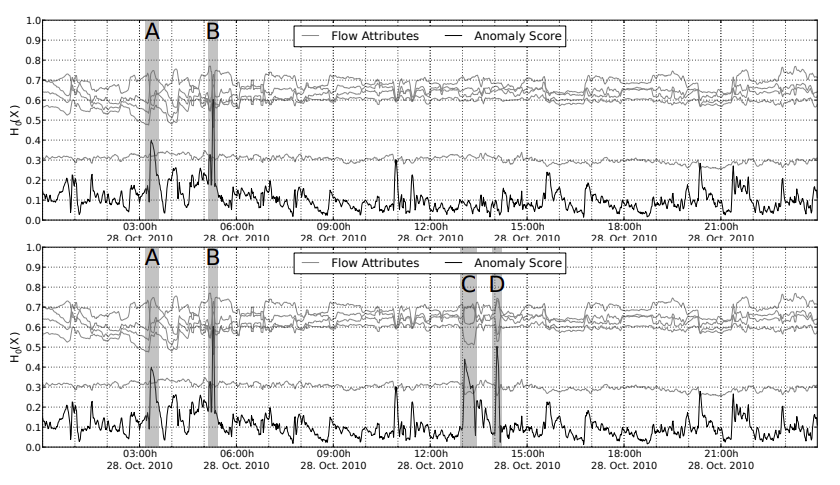
\includegraphics[scale=0.5]{./img1.png}

В качестве иллюстрации того, как это всё может остаться незамеченным традиционными средствами мониторинга: на рисунке ниже показаны три популярных
статистики трафика: количество байтов, пакетов и потоков в минуту для того же трафика, что и в предыдущем примере. Аномалии (опять же, обозначенные от A до D) исчезают в шуме.
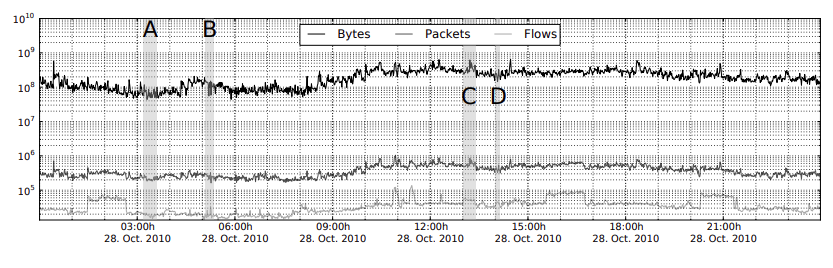
\includegraphics[scale=0.5]{./img3.png}


\begin{thebibliography}{}

\bibitem[Winter(2011)]{Win11}
Philipp Winter, Harald Lampesberger,
Markus Zeilinger, and Eckehard Hermann 2011. ``On Detecting Abrupt Changes
in Network Entropy Time Series''

\bibitem[Sharma and Sahu(2015)]{Sah15}
Sidharth Sharma, Santosh Kumar Sahu,  Sanjay Kumar Jena 2015. ``On Selection of Attributes for Entropy Based
Detection of DDoS''

\bibitem[Bhuyan and Kalita(2014)]{Bhu14}
Monowar H. Bhuyan, D. K. Bhattacharyya, J. K. Kalita ``Information Metrics for Low-rate DDoS Attack
Detection : A Comparative Evaluation''


\end{thebibliography}

\end{document}
